% vim: set textwidth=78 autoindent:

\subsection{Beschriftungsplugin}\index{Plugins!Beschriftung}

% when the revision of a section has been finalized, 
% comment out the following line:
%\updatedisclaimer

Das Plugin \toolbtntwo{labeling}{Beschriftung} bietet intelligente Beschriftung 
f�r Vektorlayer (Punkte, Linien und Polygone) und ben�tigt nur wenige Parameter. 
Dieses Plugin funktioniert auch bei On-The-Fly transformierten Layern und wird 
in Zukunft die Standard-Beschriftung in QGIS abl�sen. 

\begin{enumerate}
  \item Starten Sie QGIS und laden Sie eine Vektor Punkt-, Linien- oder Polygonlayer.
  \item Laden Sie das Plugin Beschriftung im Plugin Manager (siehe Kapitel 
  \ref{sec:load_core_plugin}), aktivieren Sie den Layer in der Legende und klicken 
  Sie dann auf das Icon \toolbtntwo{labeling}{Beschriftung} in der Werkzeugleiste.
\end{enumerate}

\minisec{Punktlayer beschriften}

Als erstes m�ssen Sie das Kontrollk�stchen \checkbox{Diesen Layer beschriften} 
aktivieren und eine Attributspalte angeben, deren Inhalt f�r die Beschriftung 
verwendet werden soll. Danach k�nnen Sie die Platzierung, den Textstil, die 
Priorit�t der Beschriftung und die Ma�stabsabh�ngige Darstellung festlegen. �ber 
weitere Kontrollk�stchen k�nnen Sie noch angeben, ob alle Teile eine mehrteiligen 
beschriftet werden sollen, ob Objekte ein Hindernis f�r die Beschriftung sein 
sollen oder nicht (siehe Abbildung \ref{fig:pointlabel}).

\begin{figure}[ht]
\begin{center}
   \caption{Intelligente Beschriftung von Vektor Punktlayern \nixcaption}\label{fig:pointlabel}\smallskip
   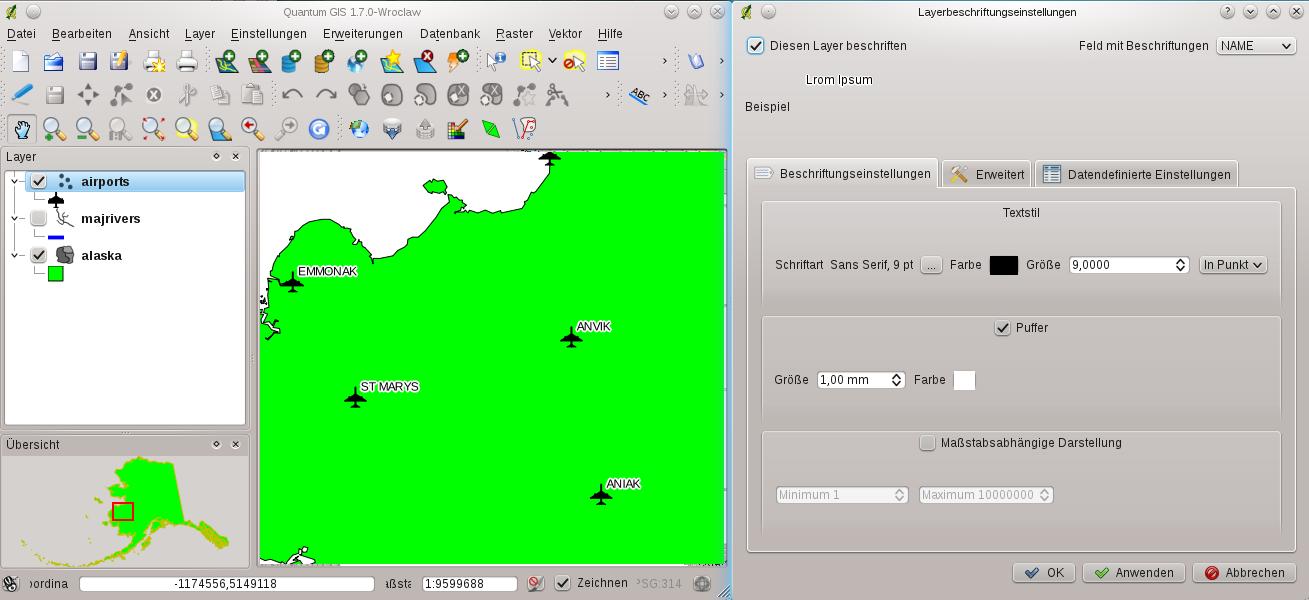
\includegraphics[clip=true, width=12cm]{label_points}
\end{center}
\end{figure}

\minisec{Linienlayer beschriften}

Als erstes m�ssen Sie das Kontrollk�stchen \checkbox{Diesen Layer beschriften}
aktivieren und eine Attributspalte angeben, deren Inhalt f�r die Beschriftung
verwendet werden soll. Danach k�nnen Sie die Platzierung, den Textstil, die
Priorit�t der Beschriftung und die Ma�stabsabh�ngige Darstellung festlegen. �ber
weitere Kontrollk�stchen k�nnen Sie noch angeben, ob alle Teile eine mehrteiligen
beschriftet werden sollen, ob sich anschlie�ende Linien verbunden werden sollen, 
um doppelte Beschriftung zu vermeide und ob Objekte ein Hindernis f�r die 
Beschriftung sein sollen oder nicht (siehe Abbildung \ref{fig:linelabel}).

\begin{figure}[ht]
\begin{center}
   \caption{Intelligente Beschriftung von Vektor Linienlayern \nixcaption}\label{fig:linelabel}\smallskip
   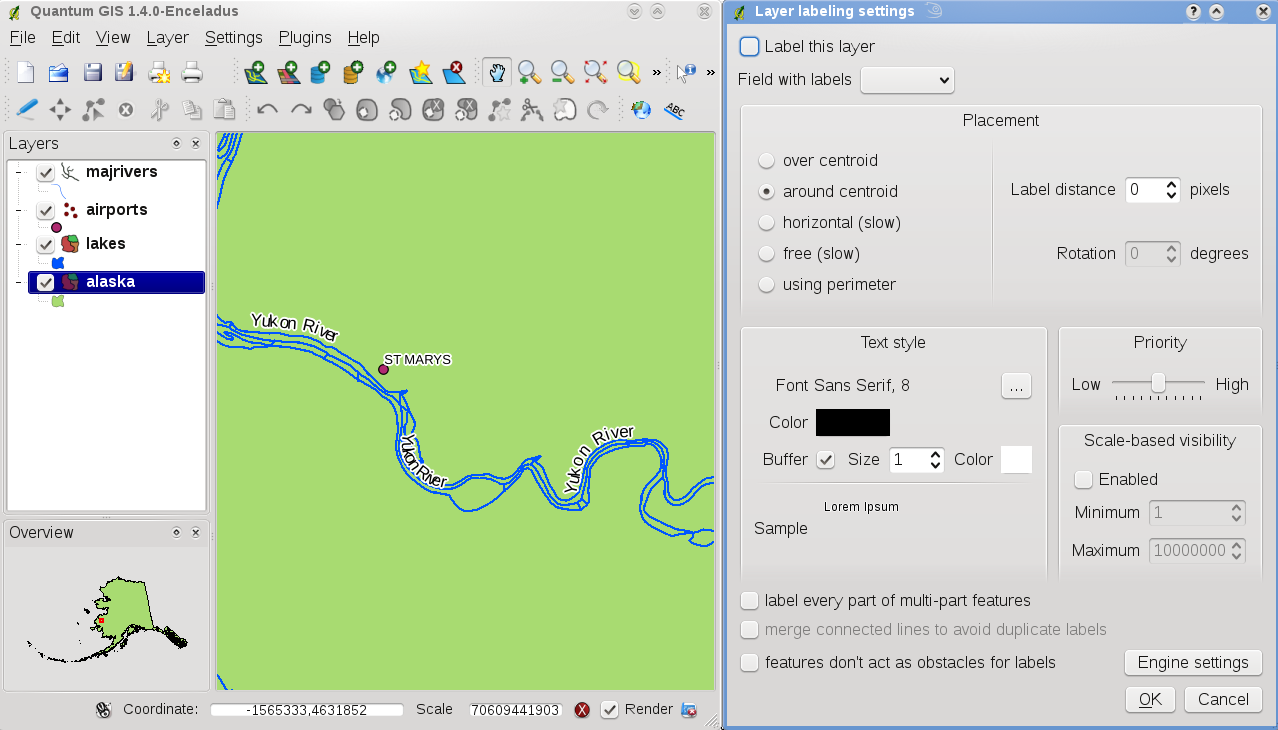
\includegraphics[clip=true, width=12cm]{label_line}
\end{center}
\end{figure}

\minisec{Polygonlayer beschriften}

Als erstes m�ssen Sie das Kontrollk�stchen \checkbox{Diesen Layer beschriften}
aktivieren und eine Attributspalte angeben, deren Inhalt f�r die Beschriftung
verwendet werden soll. Danach k�nnen Sie die Platzierung, den Textstil, die
Priorit�t der Beschriftung und die Ma�stabsabh�ngige Darstellung festlegen. �ber
weitere Kontrollk�stchen k�nnen Sie noch angeben, ob alle Teile eine mehrteiligen
beschriftet werden sollen, ob Objekte ein Hindernis f�r die Beschriftung sein
sollen oder nicht (siehe Abbildung \ref{fig:arealabel}).

\begin{figure}[ht]
\begin{center}
   \caption{Intelligente Beschriftung von Vektor Polygonlayern \nixcaption}\label{fig:arealabel}\smallskip
   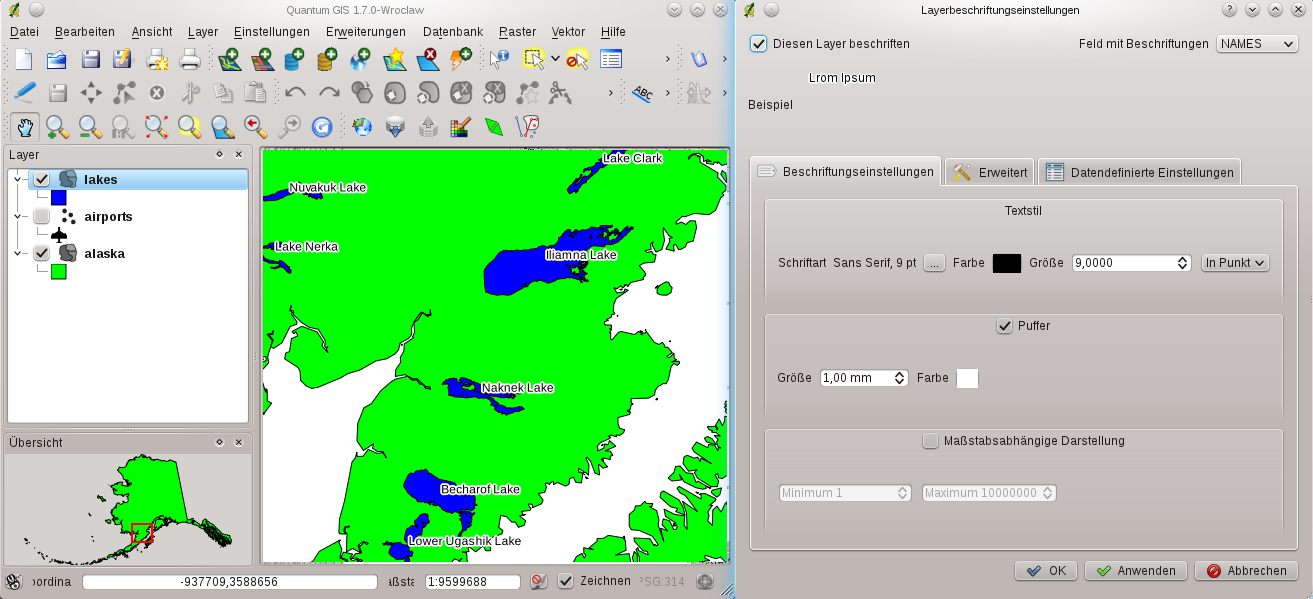
\includegraphics[clip=true, width=12cm]{label_area}
\end{center}
\end{figure}

\minisec{Beschriftungseinstellungen �ndern}

Au�erdem k�nnen Sie auf den Knopf \button{Beschriftungseinstellungen} dr�cken und 
eine Suchmethode f�r die optimale Beschriftung ausw�hlen, Zur Verf�gung steht Kette, 
Popmusik Tabu, Popmusik Kette, Popmusic Tabu Kette und FALP.
 
\begin{figure}[ht]
\begin{center}
   \caption{�ndern der Beschriftungseinstellungen \nixcaption}\label{fig:labelengine}\smallskip
   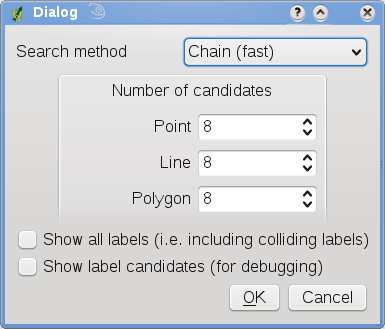
\includegraphics[clip=true, width=7cm]{label_engine}
\end{center}
\end{figure}


Dazu k�nnen Sie noch ausw�hlen, ob alle Beschriftungskandidaten angezeigt werden 
sollten (zur Fehlerbeseitigung) oder ob alle Beschriftungen dargestellt werden 
sollen, also inklusive der kollidierenden.

\newpage

